\section{Diffusion Approximation}

\label{sec:diffusion_approximation}

The previous section derived a diffusion equation from the $P_1$-equations by assuming an isotropic distribution of the radiance field for the moment closure problem. We solve this diffusion equation very efficiently using a multigrid solver similarly to Stam et al.~\cite{Stam95} and discuss the results in this section.

The multigrid solver is implemented in a straightforward fashion. However, since Stam only mentions the use of a multigrid solver very briefly, we give more details on its implementation in appendix~\ref{sec:da_solver}.

In terms of the rendering integration, it is important to note that the diffusion approximation only gives the solution to the zero moment $L^{0,0}$, which is the same as the fluence $\phi$. Higher moments are not needed, if the phase function is isotropic, as discussed in section~\ref{sec:pn_rendering_integration} and shown in equation~\ref{eq:pn_rendering_integration2}. However, in the case of an anisotropic phase function, equation~\ref{eq:pn_rendering_integration2} applies, which requires the evaluation of $\widehat{L}_m$, the full reconstruction of the truncated spherical harmonics expansion of the radiance field. For the diffusion approximation, this was derived in section~\ref{sec:da_moment_expansion_L} and resulted in equation~\ref{eq:moment_expansion_L}. While the first term is straightforward to evaluate using the zero moment from the diffusion solve, the second term requires the flux vector. This needs first to be computed using the definition, which had been derived using the isotropic moment closure in section~\ref{sec:moment_closure}, where equation~\ref{eq:diffusion_ficks_law} is used. With the definition, the first moment can be reconstructed from the gradient of the zero moment and used to evaluate $\widehat{L}_m$.

\subsection{Point Source Problem}
\label{sec:da_results_pointsource}
The solver is first run on the point source problem described in section~\ref{sec:pn_results_pointsource} and compared against the results from the $P_N$-method.
\begin{figure}[h]
\centering
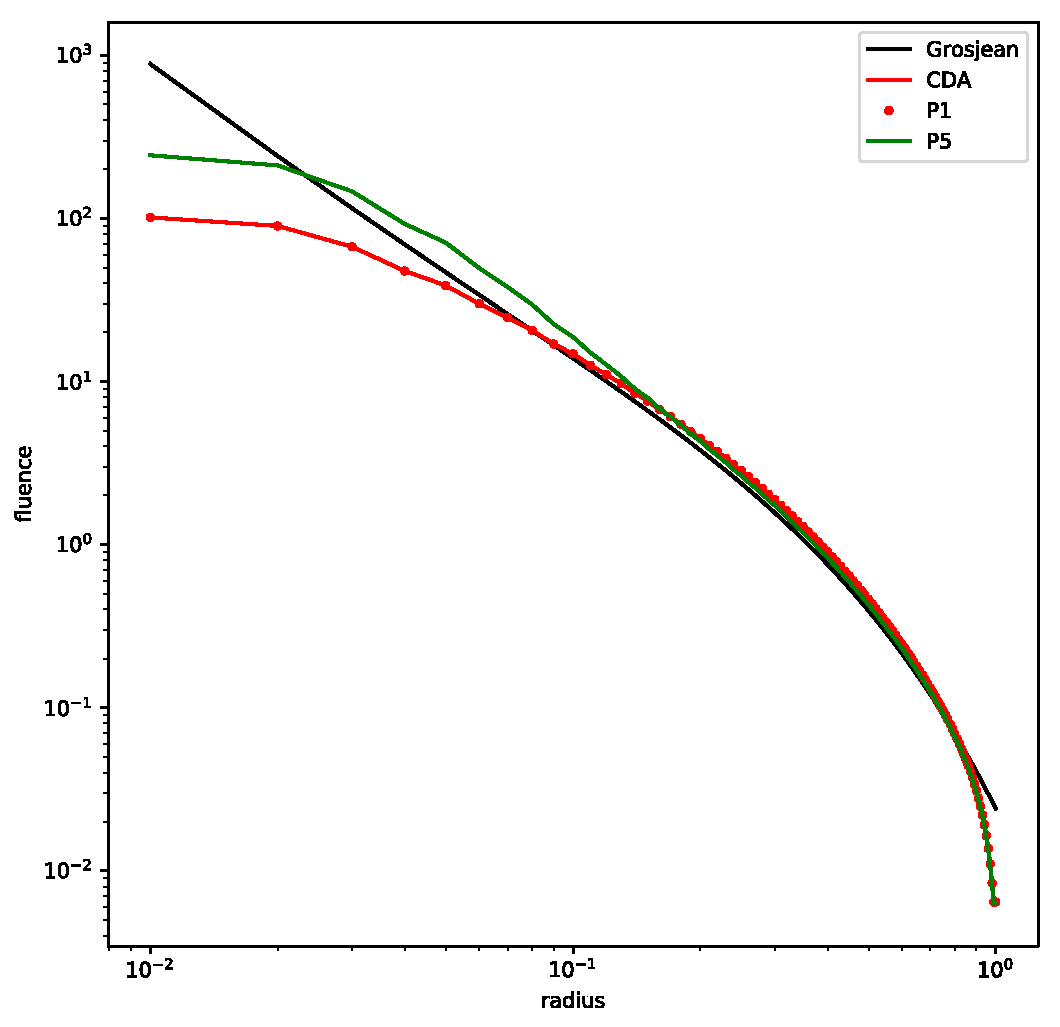
\includegraphics[width=0.8\textwidth]{05_diffusion_approximation/results/cda_result_plot_pointsource.pdf}
%\missingfigure{pointsource plots DA}
\caption{Solution of the diffusion approximation for the point source problem (red line) compared against ground truth (black), $P_1$ (red dots) and $P_5$~(green).}
\label{fig:da_results_pointsource_1}
\end{figure}

As expected, the accuracy of the $P_N$-result is better than for the diffusion approximation as soon as the truncation order of the $P_N$-method is increased. However, for the truncation order of $N=1$, identical results are shown. This is explained by the fact that the diffusion approximation is derived by collapsing the $P_1$ equations by using substitution. Therefore, the diffusion equation is mathematically equivalent to the $P_1$-equations and consequently is satisfied by the exact same solution. This result further validates that the $P_N$-solver has been implemented correctly.


\begin{figure}[h]
\centering
\begin{subfigure}[t]{0.48\columnwidth}
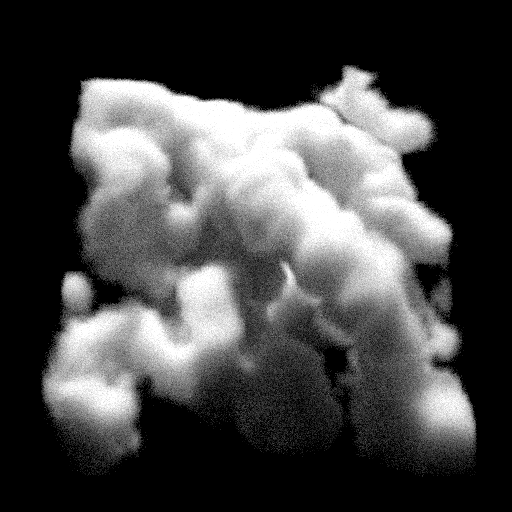
\includegraphics[width=\columnwidth]{04_pn_method/results/nebulae_ms_groundtruth.png}
\caption{Pathtraced}
\label{fig:pn_results_nebulae1_pathtraced}
\end{subfigure}
\hspace{0.01\columnwidth}
\begin{subfigure}[t]{0.48\columnwidth}
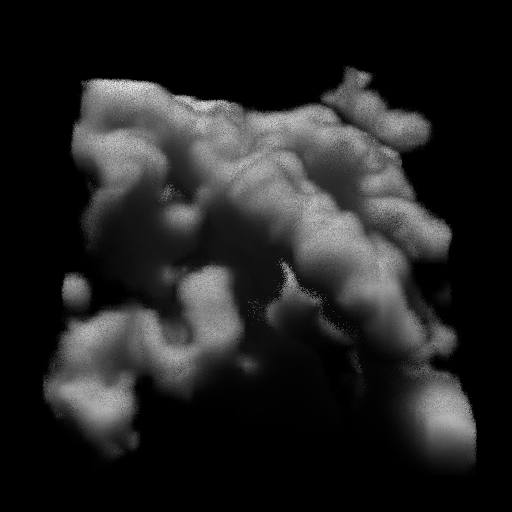
\includegraphics[width=\columnwidth]{05_diffusion_approximation/results/nebulae_ms_cda.png}
\caption{Diffusion Approximation}
\label{fig:pn_results_nebulae1_P1}
\end{subfigure}

\begin{subfigure}[t]{0.48\columnwidth}
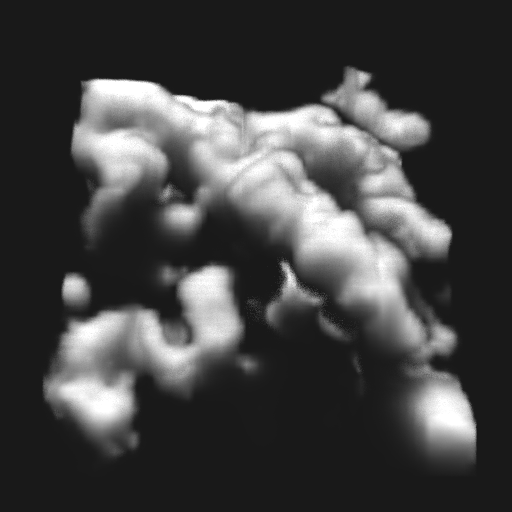
\includegraphics[width=\columnwidth]{04_pn_method/results/nebulae_p1_ms.png}
\caption{$P_1$}
\label{fig:pn_results_nebulae1_P3}
\end{subfigure}%
\hspace{0.01\columnwidth}
\begin{subfigure}[t]{0.48\columnwidth}
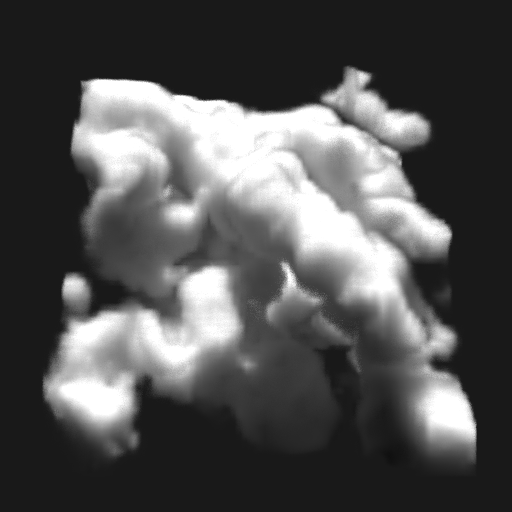
\includegraphics[width=\columnwidth]{04_pn_method/results/nebulae_p5_ms.png}
\caption{$P_5$}
\label{fig:pn_results_nebulae1_P5}
\end{subfigure}

%\vspace{-0.2in}
\caption{Diffusion approximation results for the procedural cloud dataset (multiple scattered light) compared against Monte-Carlo reference, $P_1$ and $P_2$.}
\label{fig:da_results_nebulae_1}
\end{figure}

\subsection{Procedural Cloud}
\label{sec:da_results_clouds}

Finally, the multigrid solver for diffusion is run on the procedural cloud problem from section~\ref{sec:pn_results_clouds}. The presence of vacuum regions in the dataset caused the $P_N$-method not to converge, but it was still possible to run iterations that would reduce the residual error albeit slowly. However, for the diffusion approximation, the presence of vacuum regions causes the method to break down completely, as the diffusion coefficient (equation~\ref{eq:da_D}) requires division by the extinction coefficient and therefore produces a division by zero. This aspect is easily confused, when reading the neutron transport literature. Papers such as Hansen et al.~\cite{Hansen14} state that the normal form of the $P_N$-equations can deal with voids. This is true in the sense that it does not produce a division by zero directly. However, it still is not convergent.

As with the point source problem, it is shown that the $P_1$-results, match the diffusion results while higher truncation order produces more accurate results for the $P_N$-method. In particular, the diffusion approximation (or $P_1$) fail to reproduce the illumination of the indirectly illuminated region at the bottom of the dataset.
%\begin{figure}[h]
%\centering
%\missingfigure{procedural cloud convergence plots DA P1 P5}
%\caption{TODO}
%\label{fig:da_results_nebulae_2}
%\end{figure}
